\documentclass[11pt,a4paper]{article}
\usepackage[utf8]{inputenc}
\usepackage[T1]{fontenc}
\usepackage{lmodern}
\usepackage[hyphens]{url}\urlstyle{same}
\usepackage{amsmath,amssymb}
\usepackage{geometry}
\usepackage{booktabs}
\usepackage{graphicx}
\usepackage{xcolor}
\usepackage{hyperref}
\usepackage{enumitem}
\geometry{margin=2.3cm}
\graphicspath{{../images/}}
\setlist{itemsep=2pt,topsep=3pt}
\setlength{\emergencystretch}{3em}
\newcommand{\code}[1]{\texttt{#1}}
\newcommand{\dt}{\Delta t}

\title{MultiRate.jl: findings\\[2pt]\large Partially implicit MIS methods for the compressible Euler
equations with gravity on DGSEM, terrain-following FV and cut-cell FV}
\author{}
\date{November 2026}

\begin{document}
\maketitle

\begin{abstract}
This report collects the results of the numerical experiments with MultiRate.jl in the order they
were obtained: background-free discretizations, the Agnesi hills, gravity waves, the MIS tableaus,
linear acoustics with advection after the MISDG experiments, the linearized production models and
a matrix-free analysis of the linearized step. The recurring result is that the slow part
$S = N - L$ of a split-explicit step must not contain terms whose Courant number with the large step
is large. Two instances are identified: the vertical transport of horizontal momentum by the fast
vertical velocity (Agnesi a100 and the long-channel gravity wave, $U\dt/\Delta z = 13$--$22$), and a
grid-scale mode on the steep flanks of the a1 hill (preliminary). The markdown version of these
findings is \code{docs/FINDINGS.md}; the MISDG talks are in \code{docs/talks/}.
\end{abstract}

\tableofcontents

%======================================================================
\section{The method}

The semi-discrete system is $q' = N(q)$. At the start of a large step the fast linear operator $L$
is frozen at $q^n$ (in the runs it is re-frozen every 10 steps), and $S(q) = N(q) - L q$ is the slow
part. Stage $i$ of an MIS method solves the fast system
\begin{equation}
  Z' = L Z + \sum_{j<i} \frac{\gamma_{ij}}{d_i\dt}\,\Delta Y_j + \sum_{j\le i}\frac{\beta_{ij}}{d_i}\,S(Y_j),
  \qquad Z(0) = q^n + \sum_{j<i}\alpha_{ij}\Delta Y_j,
\end{equation}
over $[0, d_i\dt]$, $d_i = \sum_j\beta_{ij}$, with $n_i = \max(1, \mathrm{round}(d_i\,n_\mathrm{sub}))$
substeps, and sets $Y_{i+1} = Z(d_i\dt)$, $\Delta Y_i = Y_{i+1} - q^n$. The paper form uses
$(s+1)\times(s+1)$ matrices; MultiRate stores $\beta = P[2{:}\mathrm{end}, 1{:}\mathrm{end}-1]$ and
$\alpha,\gamma = P[2{:}\mathrm{end},2{:}\mathrm{end}]$ (\code{mis\_from\_paper}). For $L = 0$ the
method is the Runge--Kutta method with $B = (I-\alpha-\gamma)^{-1}\beta$.

The fast integrators are \code{:verlet} (Störmer--Verlet, thermodynamic kick and momentum),
\code{:fb} (forward--backward), \code{:hevi} (horizontally explicit, vertically implicit), for FV
the Strang composition of horizontal Verlet half steps around a vertical Crank--Nicolson step,
\code{:hevi\_verlet} (DGSEM), \code{:wrf} (WRF's off-centred vertical step with divergence damping)
and, for cut cells, a Rosenbrock-W AMF step (\code{:rosenbrock\_amf}).

The spatial discretizations are DGSEM (degree 4, LMARS/entropy-conservative volume fluxes), a
terrain-following Arakawa C-grid FV with a Gal-Chen vertical coordinate, and a cut-cell C-grid FV.
All production runs use MIS4 with $n_\mathrm{sub} = 12$.

%======================================================================
\section{Discretizations without a background state}

\begin{itemize}
\item DGSEM uses the pointwise fast operator $L$ (frozen $\bar\theta$ and $\gamma p/\Theta$, as in the
  HEVI Jacobian of Artiano et al.); terrain-following FV the conservative \code{:flux} form of the
  $\Theta$ equation; cut cells \code{:donor}. None of them uses $\bar\theta(z)$.
\item FV without a hydrostatic reference $\bar p, \bar\rho$ (\code{FV\_HYDRO\_REFERENCE[] = false},
  the default): the momentum equations use full $p$ and $\rho$. The analytic hydrostatic initial
  state, sampled where the operator places the values (cut cells: the full-cell centre), is balanced
  to $O(\Delta z^2)$ (test: residual ratio $> 1.9$ between $n_z = 6$ and $12$).
\item At rest, 6\,h on the a10 grid, $\max|w|$: terrain FV $4.1\cdot10^{-3}$\,m/s ($10^{-11}$ with
  the reference), cut cells $9\cdot10^{-3}$\,m/s ($3\cdot10^{-5}$ with the reference).
\item \textbf{Ground pressure in the Gal-Chen correction} $-\partial_\eta(z_x p)$: the ground-face
  $p$ must be extrapolated from the face \emph{means} (\code{fv\_p\_sigma},
  $\tfrac32 p_1 - p_3 + \tfrac12 p_4$), so that its $O(\Delta\eta^2)$ error matches that of the
  interior means and cancels. Taking the lowest cell centre is off by $\rho g\Delta z/2$, an $O(1)$
  error ($|U_t|\approx 0.14$ at rest, independent of resolution); pointwise 2nd/3rd-order
  extrapolation is only first order. The fast operator includes the ground face the same way.
\item The flux form has a weak growing mode at rest on terrain (the $x$-flux carries $\theta$ along
  the sloped $\sigma$-surfaces, while the $\sigma$-correction uses 4-point averaged $U$;
  $\approx 5\cdot10^{-6}\,\mathrm{s}^{-1}$ on a coarse test hill, growing with horizontal resolution).
  It does not affect the Agnesi runs. \code{:advective} (state $\theta$, adjoint pressure gradient)
  removes it at the price of $\Theta$ conservation.
\end{itemize}

%======================================================================
\section{Agnesi hills}

Gallus \& Klemp (2000): $h = 400$\,m, $U = 10$\,m/s, $N = 0.01\,\mathrm{s}^{-1}$, half-widths
$a = 1, 10, 100$\,km, periodic channel of width $40a$, $T = 21.6\,a/U$; FV $200\times64$ cells, DGSEM
$50\times16$ elements of degree 4. $\max|w|$ (m/s) and the $\theta'$ range (K) at the final time:

\begin{center}
\small\begin{tabular}{lccc}
\toprule
 & DGSEM \code{hevi\_verlet} & FV terrain-following \code{hevi} & FV cut cells \code{rosenbrock\_amf}\\
\midrule
large steps & 694 & 400 & 565\\
a1   & 2.77, $-1.22\ldots0.93$ & 2.54, $-1.09\ldots0.92$ (2$\Delta x$ noise) & 2.14, $-1.08\ldots0.91$\\
a10  & 0.69, $-1.48\ldots1.65$ & 0.56, $-1.39\ldots1.55$ & 0.58, $-1.43\ldots1.58$\\
a100 & 0.064, $-1.49\ldots1.70$ & 0.056, $-1.40\ldots1.57$ & 0.057, $-1.43\ldots1.61$\\
\bottomrule
\end{tabular}
\end{center}

\begin{itemize}
\item \textbf{a100 and the vertical momentum transport.} The vertical transport of horizontal
  momentum by the fast vertical mass flux, $-\partial_z(\bar u\,W')$, must be in the implicit
  vertical $L$ (\code{DG\_VADV\_FAST}, \code{FV\_VADV\_FAST}). Left in $S$ it couples the large step
  to the vertical acoustics through the vertical Courant number $U\dt/\Delta z$ (a1 0.1, a10 1.3,
  a100 13 for DGSEM, 22 for FV), and a100 blows up. $\partial N/\partial q$ has no growing mode: this
  is a stability limit of the explicit part of MIS, not of the spatial discretization. The term is
  put into $L$ for $U\dt/\Delta z > 4$. A split-form linearization of $L$ (\code{DG\_SPLIT\_FAST})
  makes $N - L$ vanish at rest but changes neither stability nor solution; the simple pointwise $L$
  is kept. For FV, $L$ must in addition be skew.
\item \textbf{DGSEM with \code{hevi\_verlet}} runs all three hills at the regular horizontal acoustic
  step (a100: $d\tau = 26$\,s, $\dt = 313$\,s), about 16 times fewer steps than \code{hevi}.
\item \textbf{Cut cells:} \code{hevi} and \code{rosenbrock\_amf} give the same solutions; AMF also runs
  at the large steps of the MATLAB reference ($\dt = 20$\,s for a1, 100\,s for a10). Its fast-step
  CFL is 0.65 of the regular-grid limit (explicit horizontal acoustics inside the W-method).
  Open: a warm layer of $\approx0.35$\,K in the lowest cells downstream of the hill (a10).
\item \textbf{a1, terrain FV:} 2$\Delta x$ noise near the ground at the default step
  $\dt = 5.4$\,s. It disappears with half the slow step (\code{NSUB=6}, same $d\tau$,
  $\max|w| = 2.41$), so it is a slow-step limit for terrain terms in $N - L$, not a spatial defect.
  It is also present with the hydrostatic reference and with the \code{:advective} form. At twice
  the resolution the default step blows up; \code{NSUB=6} is stable (2.68). See
  Section~\ref{sec:matfree}.
\item Runs with $U\ne0$ without the reference drift in mass by $\approx2.5\cdot10^{-5}$
  ($3.7\cdot10^{-7}$ with it), attributed to the sponge relaxing to a $q_0$ that is not a discrete
  equilibrium; not investigated further.
\end{itemize}

\begin{figure}[ht]
\centering
\begin{tabular}{@{}c@{\,}c@{\,}c@{}}
DGSEM & FV terrain-following & FV cut cells\\
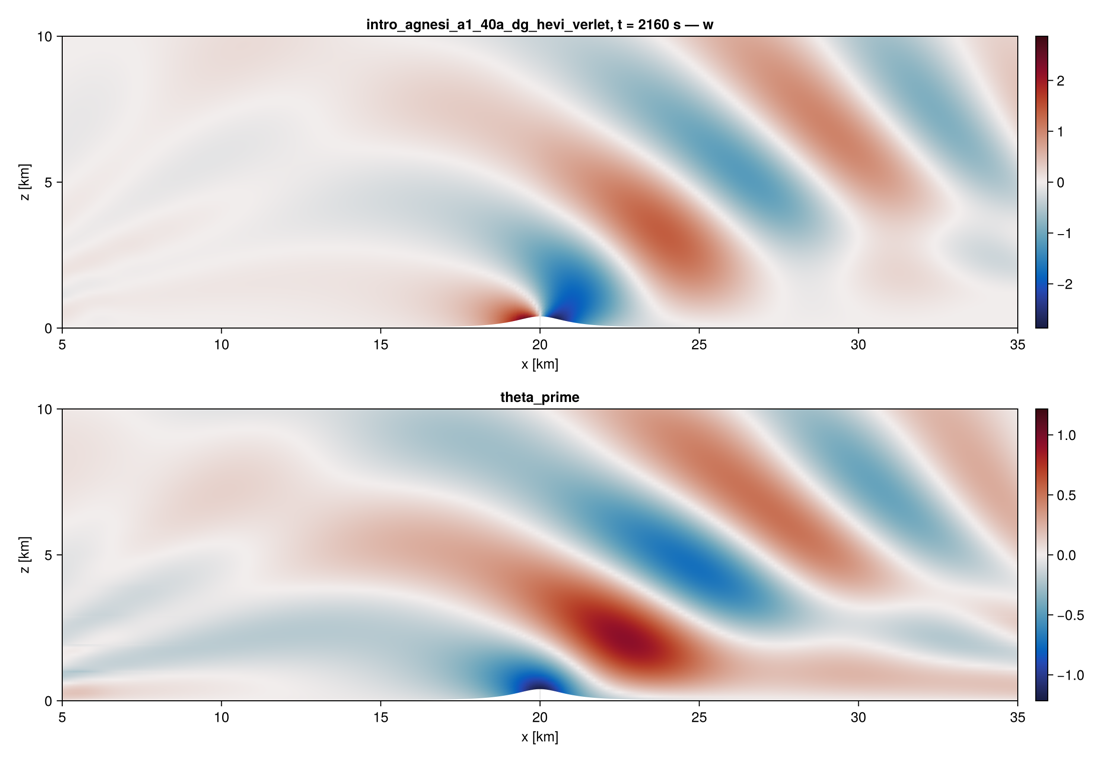
\includegraphics[width=0.32\textwidth]{agnesi_a1_dg.png} &
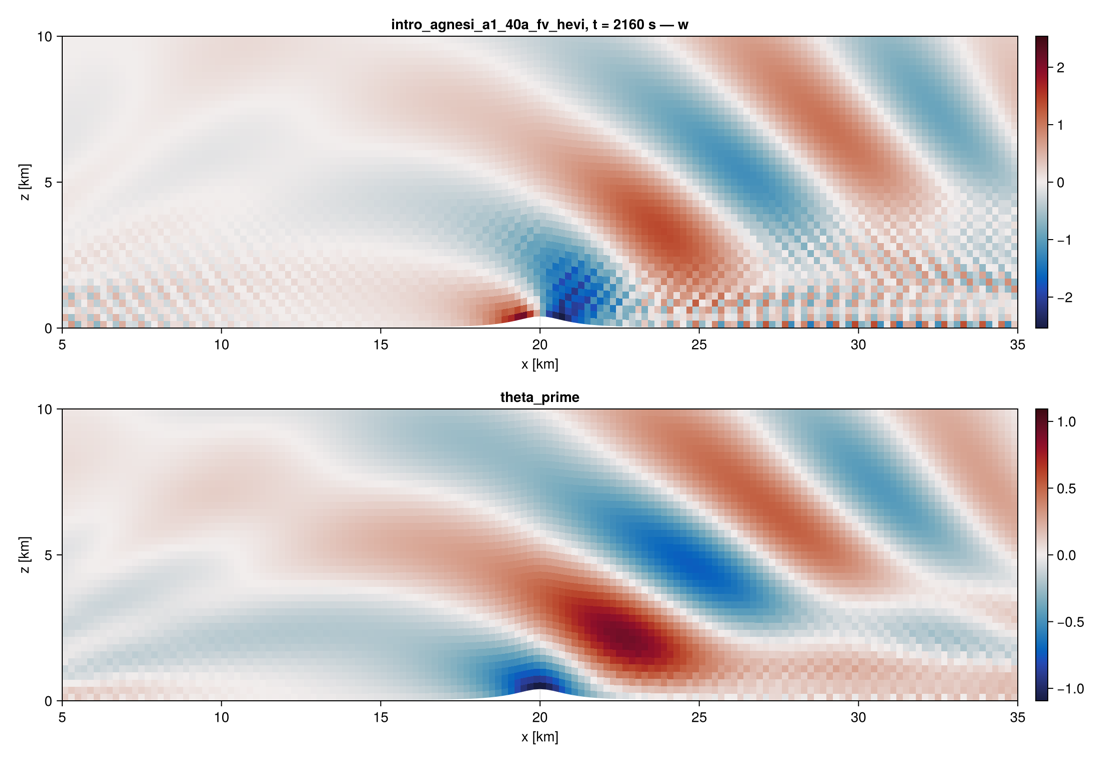
\includegraphics[width=0.32\textwidth]{agnesi_a1_fv.png} &
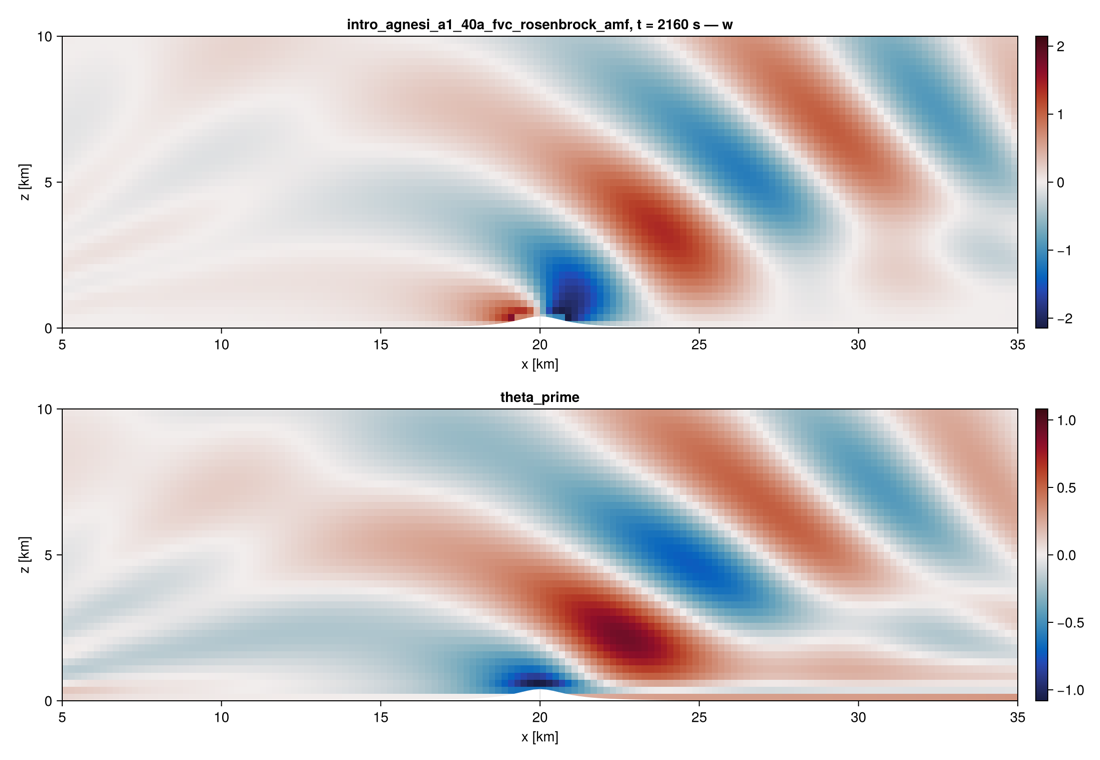
\includegraphics[width=0.32\textwidth]{agnesi_a1_fvc.png}\\
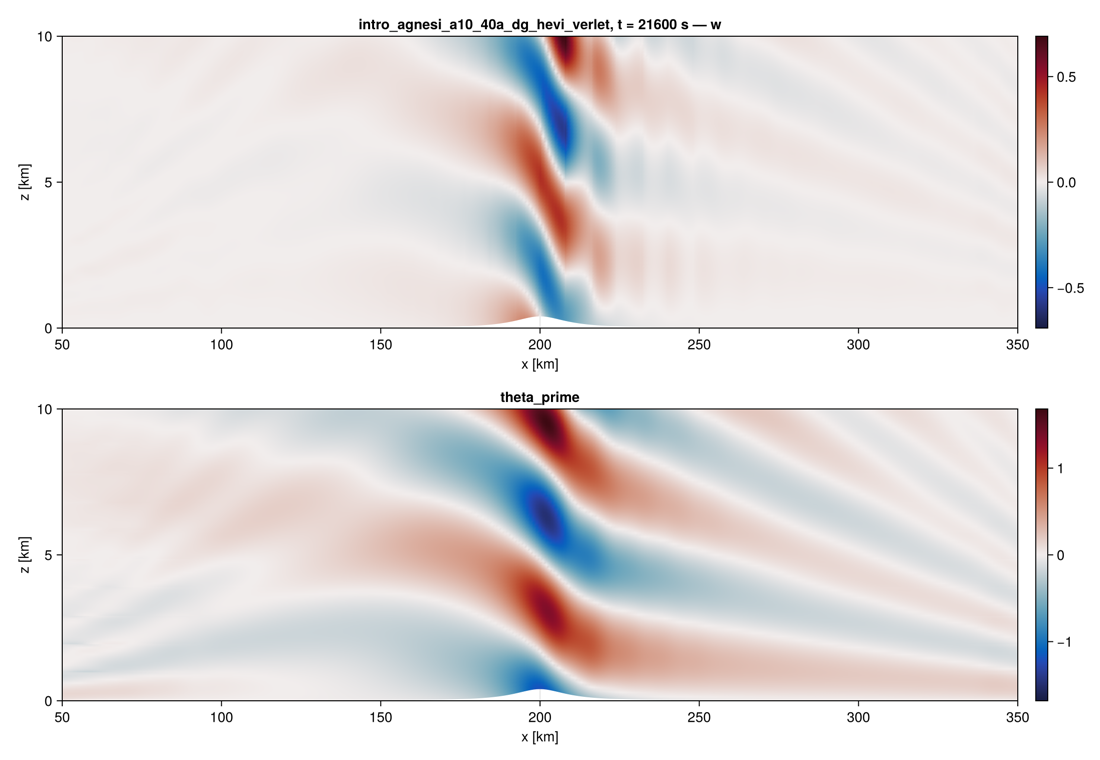
\includegraphics[width=0.32\textwidth]{agnesi_a10_dg.png} &
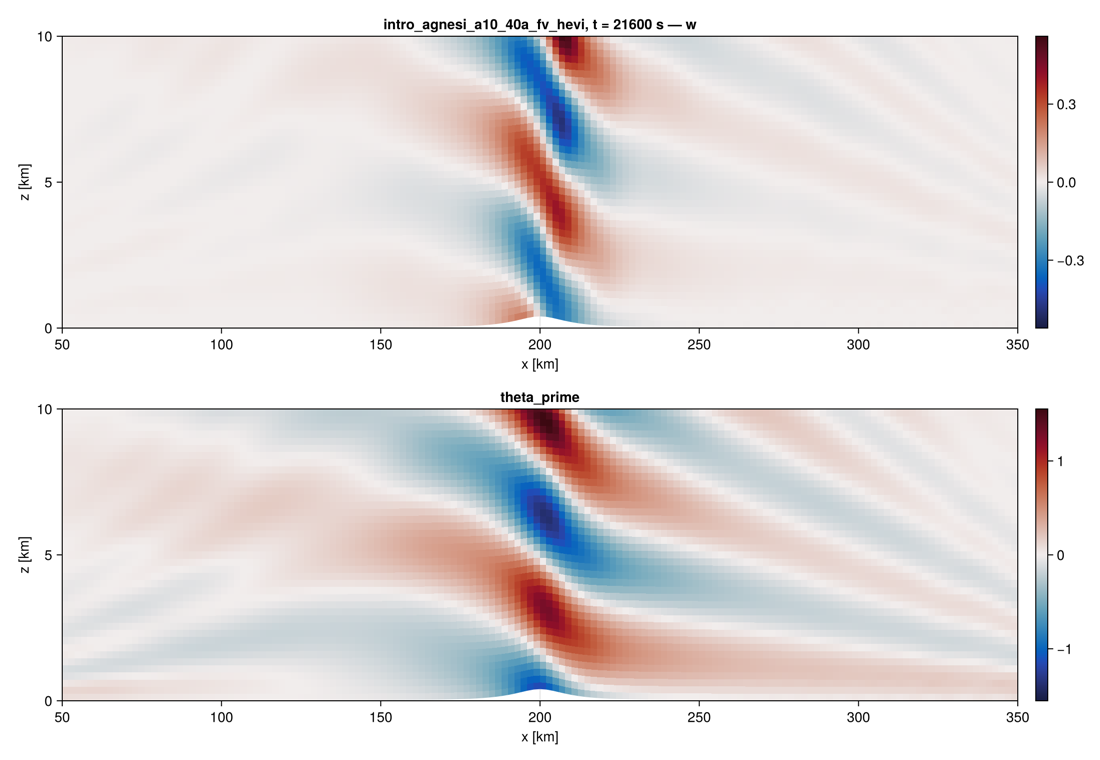
\includegraphics[width=0.32\textwidth]{agnesi_a10_fv.png} &
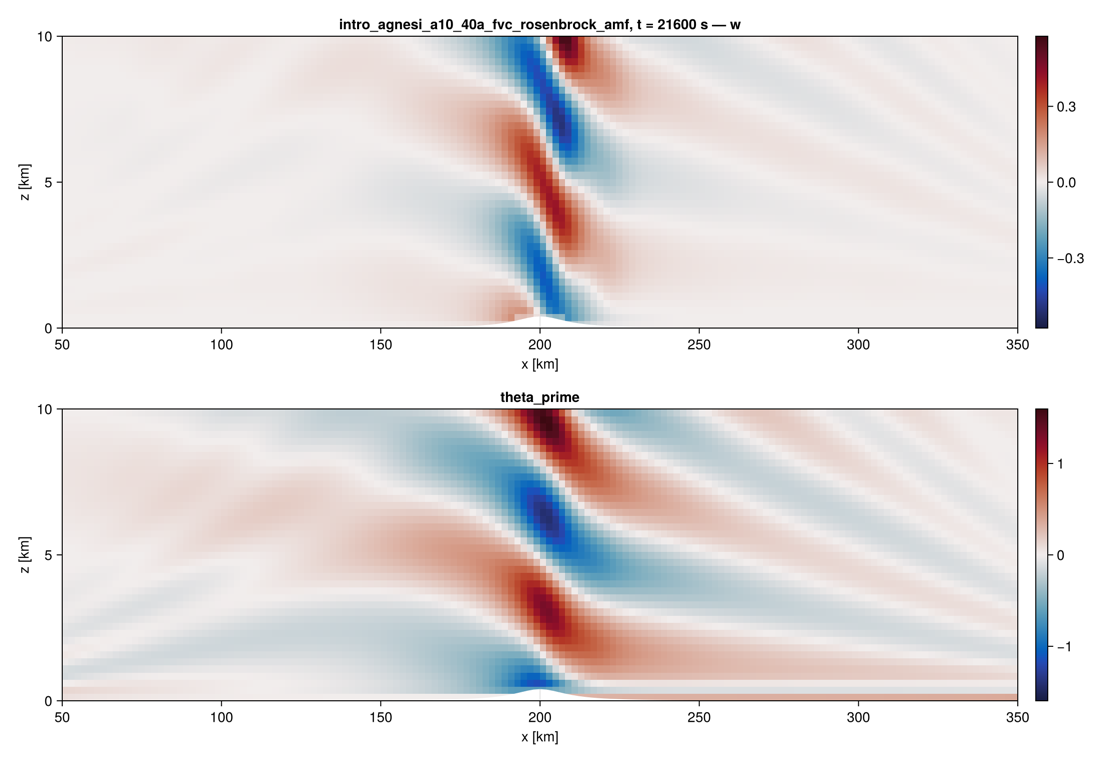
\includegraphics[width=0.32\textwidth]{agnesi_a10_fvc.png}\\
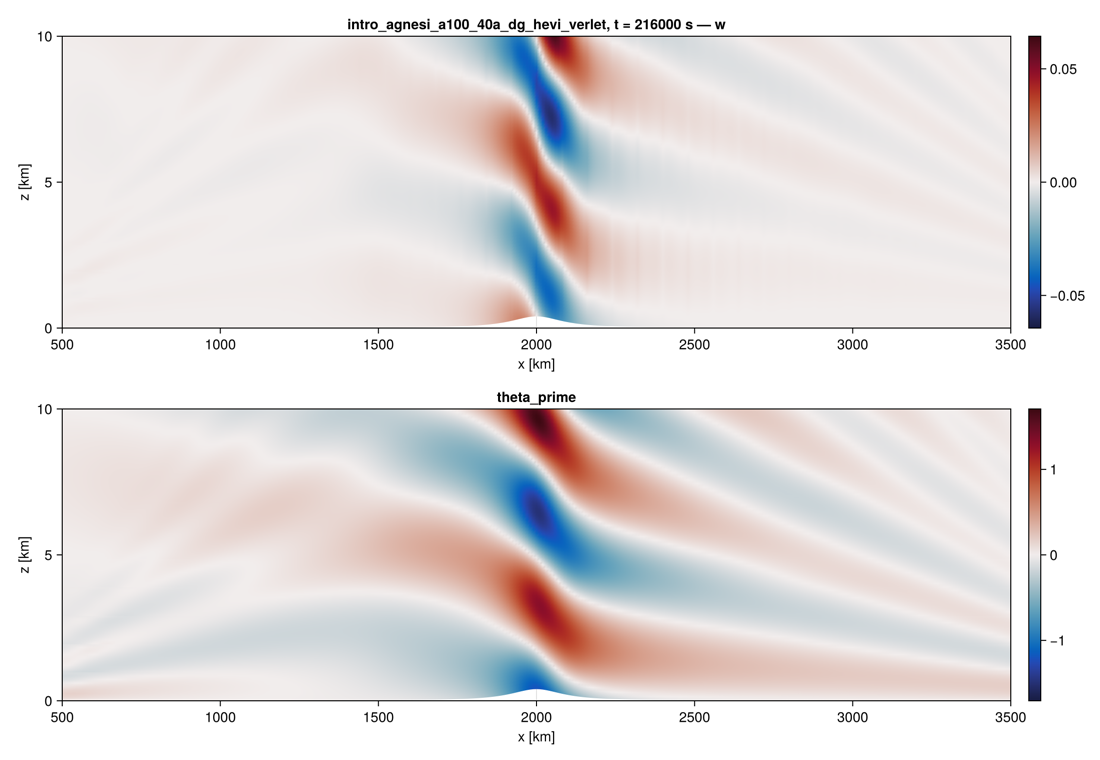
\includegraphics[width=0.32\textwidth]{agnesi_a100_dg.png} &
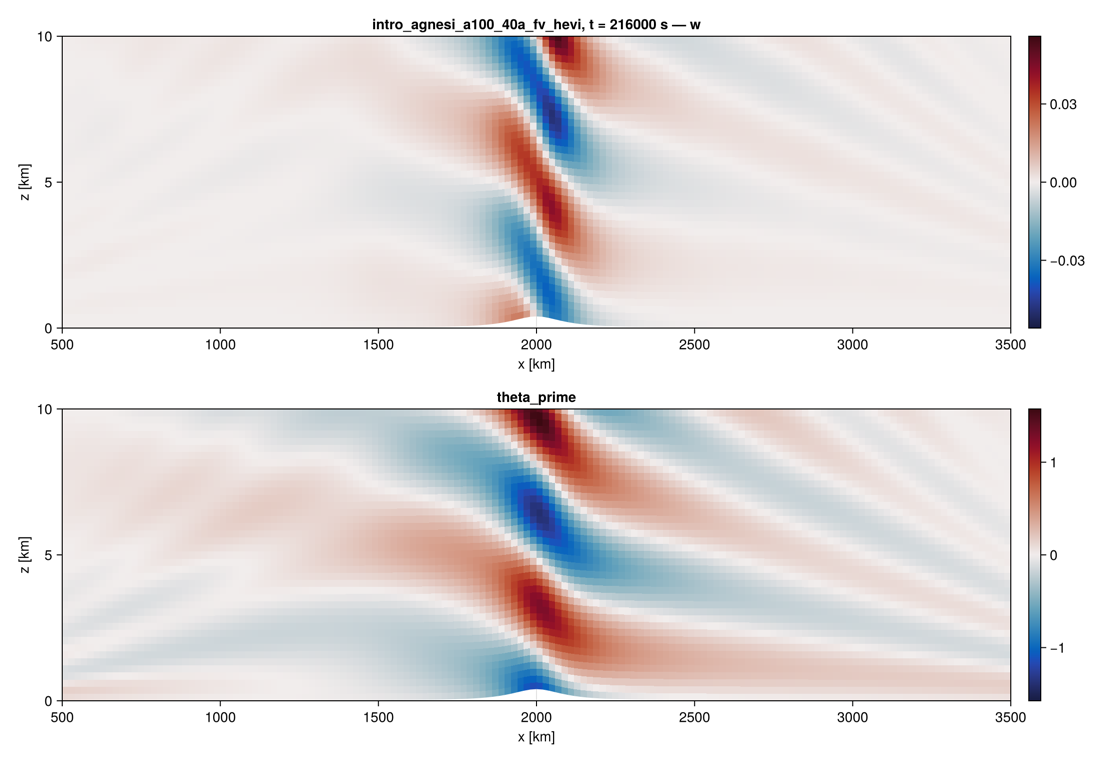
\includegraphics[width=0.32\textwidth]{agnesi_a100_fv.png} &
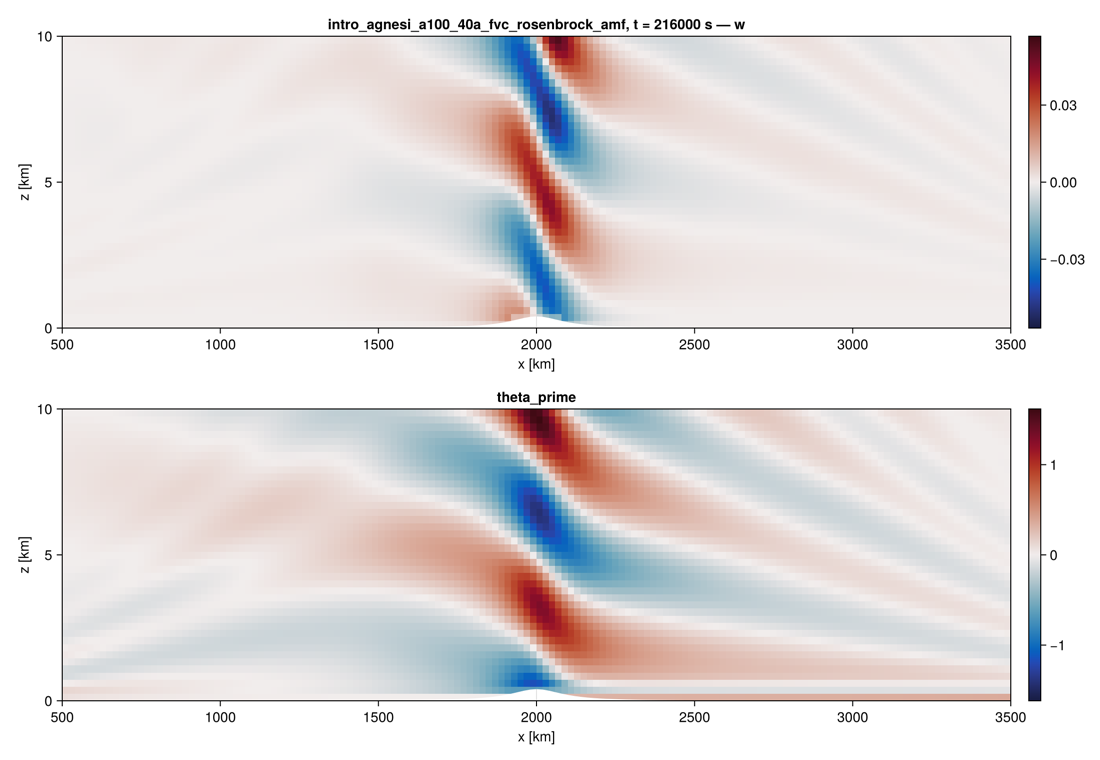
\includegraphics[width=0.32\textwidth]{agnesi_a100_fvc.png}
\end{tabular}
\caption{Agnesi hills a1 (top), a10, a100 (bottom): $w$ and $\theta'$ at the final time.}
\end{figure}

\begin{figure}[ht]
\centering
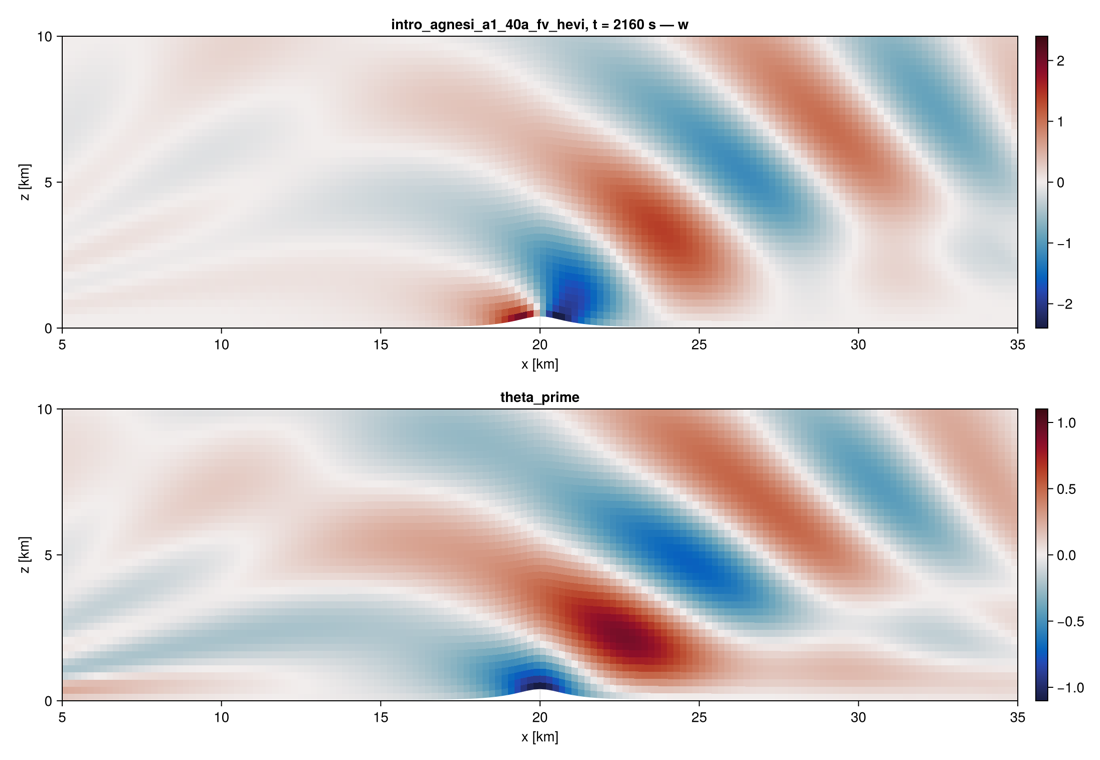
\includegraphics[width=0.6\textwidth]{agnesi_a1_fv_halfstep.png}
\caption{Terrain-following FV, a1, half the slow step (\code{NSUB=6}): the ground noise of the
default step is gone.}
\end{figure}

%======================================================================
\section{Gravity waves}

Skamarock \& Klemp (1994), flat ground:\\ \code{euler2d\_gravity\_wave.jl} (300\,km) and
\code{euler2d\_gravity\_wave\_long.jl} (6000\,km, $a = 100$\,km, $\Delta x = 20$\,km,
$\Delta z = 625$\,m, $U = 20$\,m/s, $T = 60000$\,s), MIS4, \code{hevi}, $n_\mathrm{sub}=12$.

\begin{itemize}
\item 300\,km: DGSEM and FV symmetric ($\theta'$ maxima $2.73/2.72\cdot10^{-3}$\,K DGSEM,
  $3.78/3.32\cdot10^{-3}$\,K FV).
\item 6000\,km, FV at the default step $\dt = 540$\,s ($N\dt\approx5.4$, $U\dt/\Delta x = 0.54$,
  $c\dt/\Delta x\approx9.5$): asymmetric packets ($\theta'$ maxima $2.2$ and $9.0\cdot10^{-3}$\,K) with
  grid-scale noise between them. The same with the hydrostatic reference, with the commit before the
  background was removed and with both fast solvers. With \code{NSUB=3} ($\dt = 135$\,s, same
  $d\tau$) the packets are symmetric, so the error comes from the slow step. DGSEM is clean.
\item \textbf{Cause and fix} (Section~\ref{sec:linprod}): $-\partial_z(\bar u W')$ was in $S$ although
  $U\dt/\Delta z\approx17$; the production drivers did not apply the vadv criterion of the Agnesi
  driver. With \code{set\_vadv!} (now in all drivers) the default step gives $\theta'$ maxima
  $5.34/5.29\cdot10^{-3}$\,K, asymmetry $4.4\cdot10^{-4}$\,K ($6.9\cdot10^{-3}$\,K before). The
  300\,km case ($U\dt/\Delta z = 2.1$) and DGSEM (0.6) are unchanged.
\item The uniform $\approx10^{-3}$\,K warm offset of $\theta'$ is also present for a 100 times
  smaller perturbation and for $U = 0$: a diagnostic offset of $\theta'$ against $\bar\theta(z)$ at
  the cell centres, not part of the wave.
\end{itemize}

\begin{figure}[ht]
\centering
\begin{tabular}{@{}c@{\,}c@{}}
DGSEM & FV\\
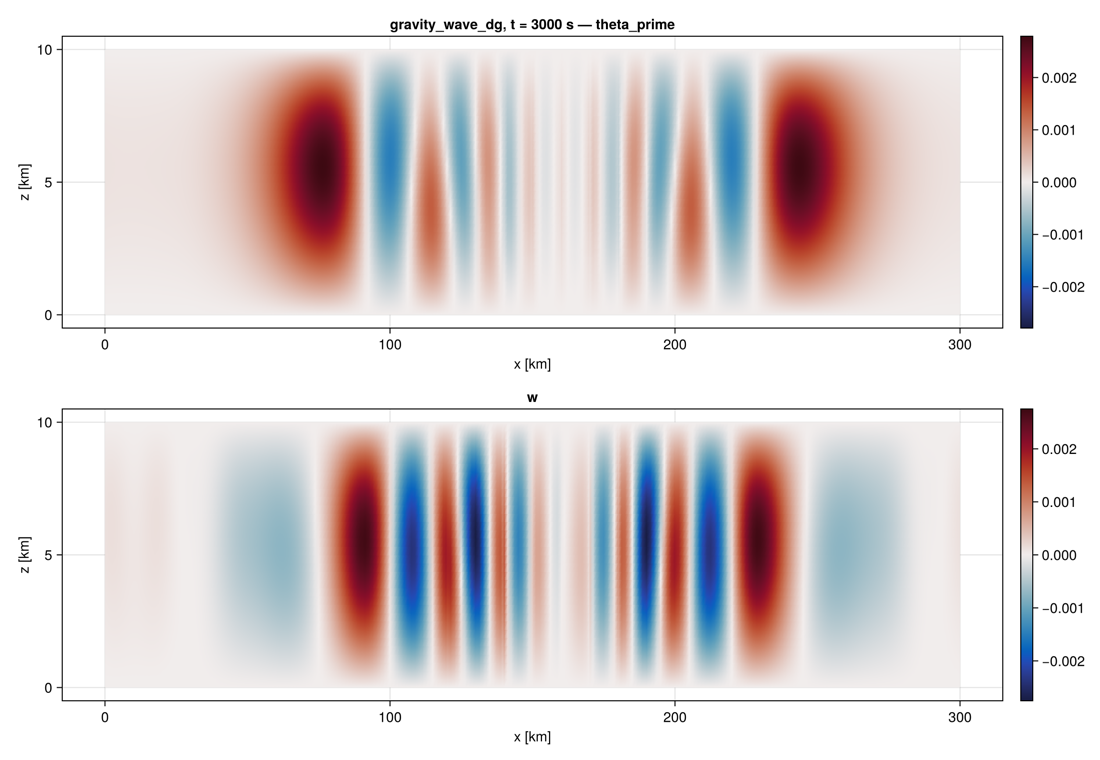
\includegraphics[width=0.48\textwidth]{gravity_wave_dg.png} &
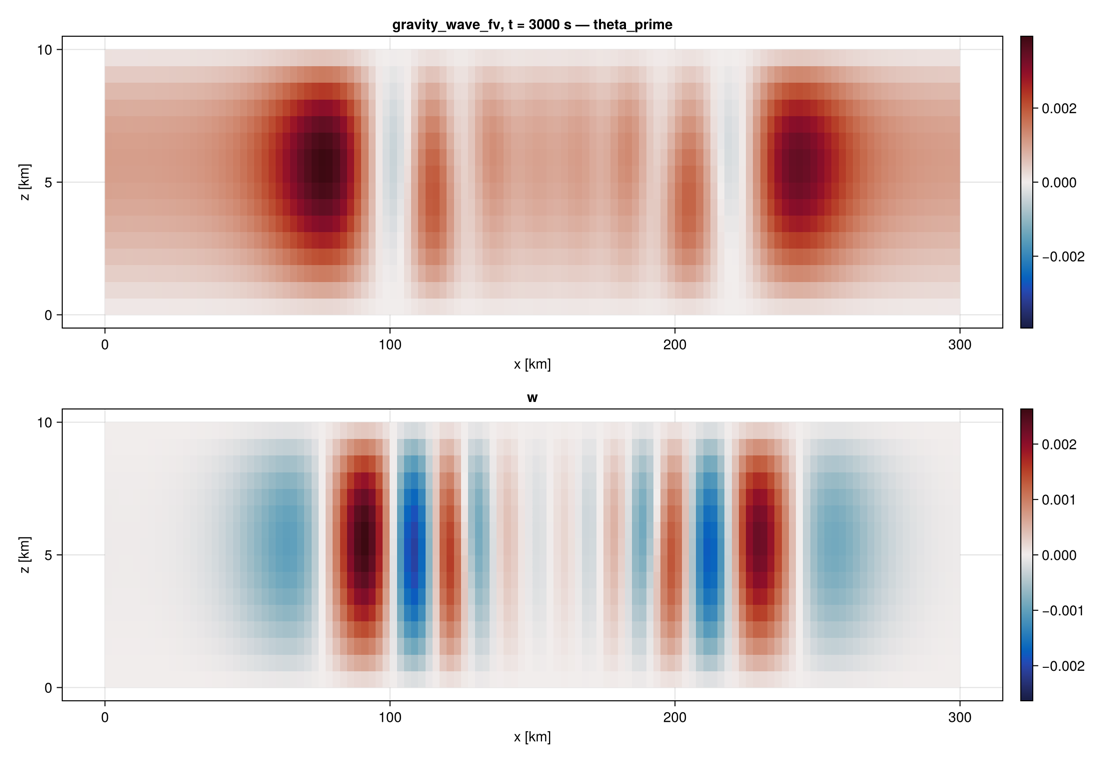
\includegraphics[width=0.48\textwidth]{gravity_wave_fv.png}\\
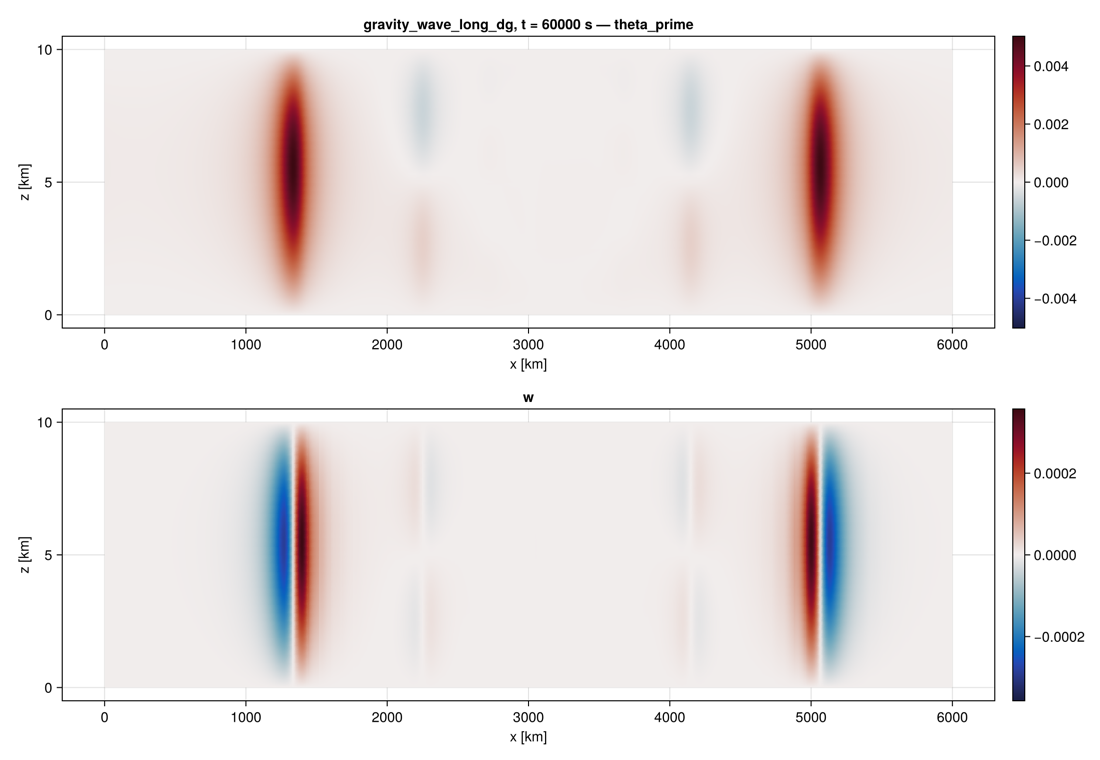
\includegraphics[width=0.48\textwidth]{gravity_wave_long_dg.png} &
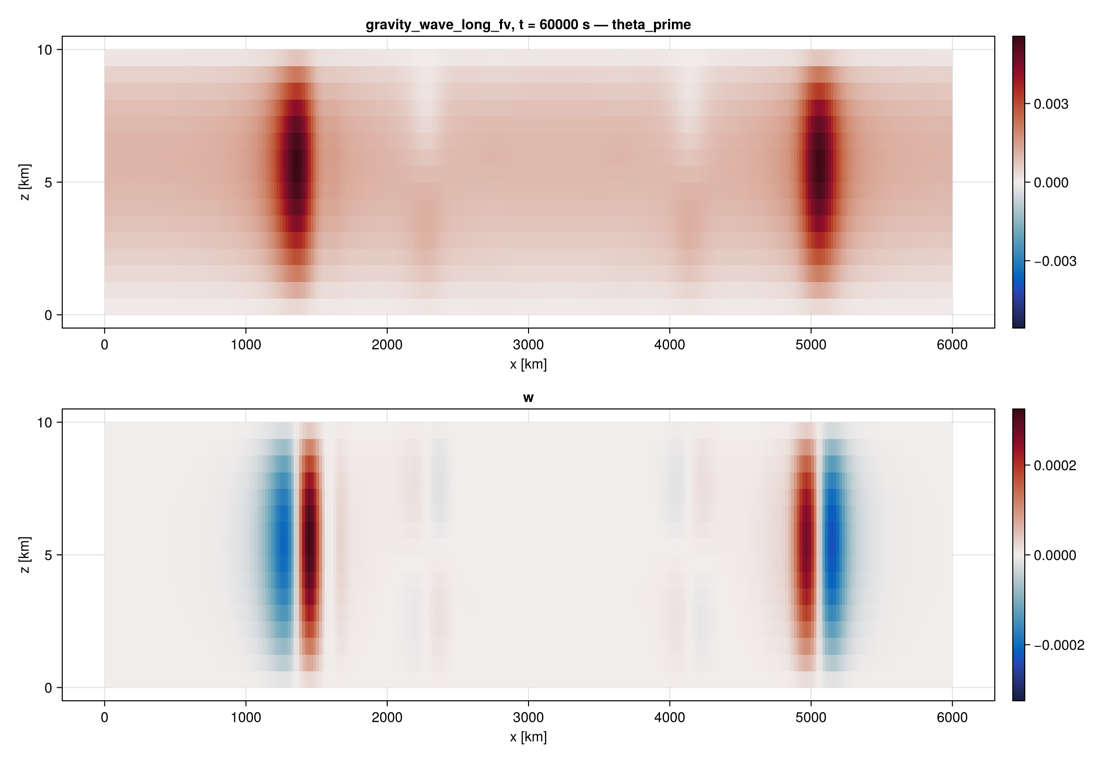
\includegraphics[width=0.48\textwidth]{gravity_wave_long_fv.png}
\end{tabular}
\caption{Gravity waves, $\theta'$ and $w$: 300\,km channel at $t = 3000$\,s (top), 6000\,km channel at
$t = 60000$\,s (bottom; FV with the vertical momentum transport in $L$).}
\end{figure}

%======================================================================
\section{MIS tableaus}

\code{TimeStepping.mis\_observed\_order} computes the order with exact fast stages (augmented
exponential) on a problem where $L$ and $S$ do not commute,
$L = \begin{pmatrix}0&4\\-4&0\end{pmatrix}$,
$G(q) = (0.5\sin q_1 + q_2^2,\ -0.3q_1q_2 + \cos q_1)$; \code{rk\_order} gives the order for $L = 0$.

\begin{center}
\begin{tabular}{lccccccc}
\toprule
 & WSRK3 & MIS2 & MIS3C & MIS4 & MIS4a & MIS\_KW3 & MIS54\\
\midrule
RK order ($L = 0$) & 2 & 2 & 3 & 3 & 3 & 3 & 4\\
MIS order & 2 & 2 & \textbf{2} & 3 & 3 & 3 & 4\\
fast time $\sum_i d_i$ & 1.83 & 1.19 & 1.19 & 1.44 & 1.47 & 1.00 & 1.88\\
\bottomrule
\end{tabular}
\end{center}

\begin{itemize}
\item MIS3C (coefficients as in ClimaTimeSteppers.jl) is only second order once $L\ne0$: a
  coupling condition fails. To be checked against Knoth \& Wensch (2014).
\item MIS\_KW3 is built from the Knoth--Wolke RK3 tableau; MIS54 is from Bauer \& Knoth (2021), with
  the coefficients of MISDG. MIS54 is fourth order and runs in the FV gravity-wave test.
\end{itemize}

%======================================================================
\section{Linear acoustics with advection}

\code{MultiRate.LinearAnalysis} treats a linear problem $q' = Nq$ with fast part $L$ as a model of
the TimeStepping interface. \code{step\_matrix} runs the production \code{mis\_step!} and fast loops
on unit vectors, or uses exact fast stages. A Fourier mode with complex symbol $A$ becomes the real
model $\begin{pmatrix}\Re A&-\Im A\\ \Im A&\Re A\end{pmatrix}$. Script:
\code{examples/linear\_analysis/mis\_stability.jl}. These are the experiments of the MISDG talk
(\code{docs/talks/misdg}).

\begin{itemize}
\item \textbf{Knoth--Wensch test} (C-grid, 2nd-order acoustics, 3rd-order upwind advection, exact
  fast stages): pure advection is stable to $C_\mathrm{adv} = 1.63$ (3-stage methods) and 2.06
  (MIS54). Undamped WSRK3 is unstable from $C_\mathrm{sound}\approx3.2$, MIS\_KW3 from $\approx2$
  (and for any $C_\mathrm{sound}$ at $C_\mathrm{adv} = 1$). MIS4a and MIS54 are stable on the whole
  box $C_\mathrm{sound}\le12$.
\item \textbf{MISDG grid} (4th-order staggered acoustics, 5th-order upwind advection,
  $C_\mathrm{adv} = C_\mathrm{sound}/7$), exact fast stages: WSRK3 stable to $C_\mathrm{sound} = 2.75$,
  MIS4 beyond 14, MIS4a to 12, MIS54 to 14. MIS\_KW3 is weakly unstable for every $C_\mathrm{sound}$
  ($\rho - 1 = 7\cdot10^{-6}$ at $C_\mathrm{sound} = 1$), as in MISDG.
\item \textbf{Fast loops}, $n_\mathrm{sub} = 12$: \code{:verlet} and \code{:fb} converge to the
  exact-stage result as $d\tau\to0$ (orders 2 and 1). At $C_\mathrm{sound} = 10$ the Verlet substep
  exceeds its own limit for every tableau. \code{:fb} makes MIS4 and MIS54 weakly unstable at
  $C_\mathrm{sound} = 3$--7, \code{:verlet} does not. WRF divergence damping (\code{:wrf}) stabilizes
  WSRK3 up to $C_\mathrm{sound} = 7$.
\item \textbf{Pulse convergence} (1D pressure pulse, exact fast stages): orders 2 (WSRK3), 3 (MIS4a),
  4 (MIS54).
\item Consequence: acoustics with advection does not explain the slow-step limits of the Agnesi and
  gravity-wave runs; MIS4 and MIS4a are stable far beyond the Courant numbers of those runs.
\end{itemize}

\begin{center}
\begin{tabular}{lcccc}
\toprule
MISDG grid, $C_\mathrm{adv} = C_\mathrm{sound}/7$ & WSRK3 & MIS4 & MIS4a & MIS54\\
\midrule
stable up to $C_\mathrm{sound}$ (exact fast stages) & 2.75 & $>14$ & 12 & 14\\
with \code{:wrf}, $n_\mathrm{sub} = 12$ & 7 & 7 & 7 & 7\\
pulse convergence order & 2 & 3 & 3 & 4\\
\bottomrule
\end{tabular}
\end{center}

\begin{figure}[ht]
\centering
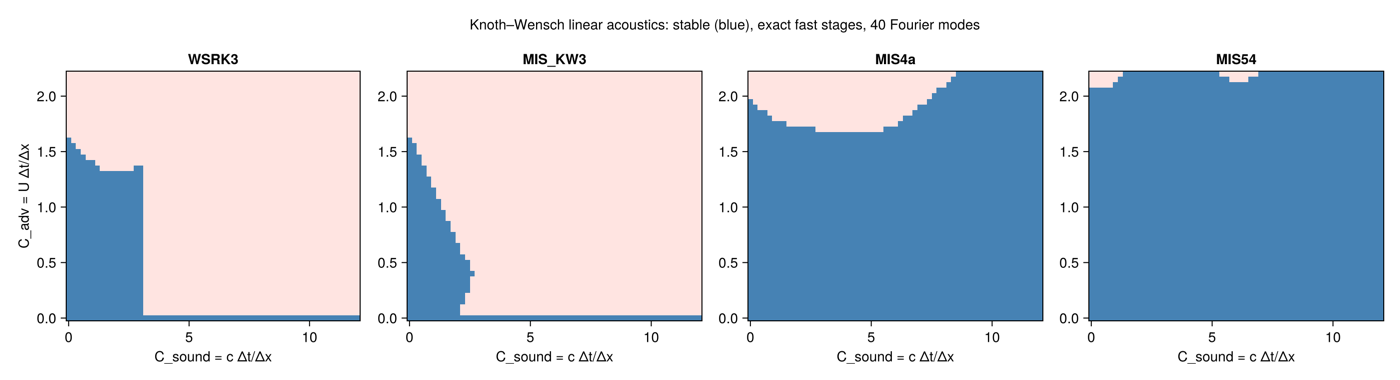
\includegraphics[width=\textwidth]{mis_stability_kw.png}\\[4pt]
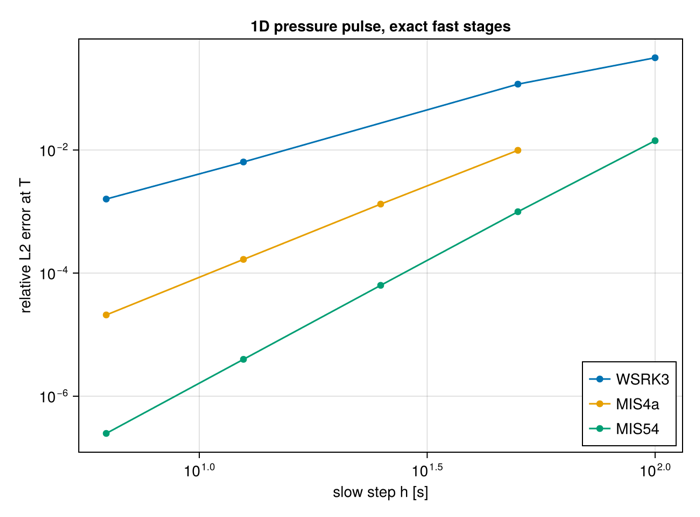
\includegraphics[width=0.55\textwidth]{mis_pulse_convergence.png}
\caption{Top: Knoth--Wensch stability regions over $(C_\mathrm{sound}, C_\mathrm{adv})$, stable in
blue, exact fast stages. Bottom: 1D pressure pulse, relative $L^2$ error against the slow step.}
\end{figure}

%======================================================================
\section{Linearized production models: the long-channel failure}\label{sec:linprod}

Script \code{examples/linear\_analysis/fv\_gravity\_wave\_split.jl}. The flat FV model is invariant
under shifts in $x$. \code{LinearAnalysis.linearized\_mode\_model} builds, per horizontal Fourier mode,
the $63\times63$ column blocks of the Jacobian $J$ of \code{rhs\_nonlinear!} (central differences),
of the frozen fast operator $L$ and of its vertical part; \code{step\_matrix} runs the production MIS
step on them. The eigenvalues of all blocks together equal those of the full fast matrix (test).

\paragraph{Steps that led to the cause.}
\begin{enumerate}
\item The real FV run is linear in the amplitude: with $\Delta\theta = 10^{-4}$ instead of
  $10^{-2}$ the asymmetry scales by $10^{-2}$. With $U = 0$ it vanishes ($10^{-5}$\,K).
\item A constant-coefficient model on the FV grids (\code{boussinesq\_symbols}: compressible
  Boussinesq, C-grid, Lorenz grid, rigid lid, buoyancy and acoustics in $L$, advection in $S$) is
  accurate at $\dt = 540$\,s (error $1.5\cdot10^{-4}$ of a $4.5\cdot10^{-3}$\,K packet). Moving the
  advection of any rows between $L$ and $S$ changes this by at most 1.4\,\%. The failure is not in the
  generic acoustic--gravity--advection problem.
\item The linearized production FV reproduces the nonlinear run ($\theta'$ maxima
  $1.319/8.017\cdot10^{-3}$\,K against $1.320/8.022\cdot10^{-3}$\,K). With exact fast stages the error
  remains, so it is the slow-step coupling; the \code{:hevi} loop adds instability
  ($\max|\lambda| = 1.15$ at $4\Delta x$--$8\Delta x$).
\item Moving rows of $S$ into $L$ (exact fast stages): the horizontal-momentum rows reduce the error
  from $1.67\cdot10^{-3}$ to $2.8\cdot10^{-5}$\,K, the $\Theta$ rows do nothing; writing $L$'s mass and
  $\Theta$ fluxes with the perturbation momentum does nothing either.
\item The stiff part of the momentum rows of $S$ is $-\partial_z(\bar u W')$ with coefficient
  $\bar u\dt/\Delta z\approx17$, the term \code{FV\_VADV\_FAST} puts into $L$.
\end{enumerate}

\begin{center}
\begin{tabular}{llcccc}
\toprule
$L$ & fast & $\dt$ [s] & packets [$10^{-3}$\,K] & max err [K] & $\max|\lambda|$\\
\midrule
as in the driver (no vadv) & exact & 540 & 6.13 / 2.80 & $1.7\cdot10^{-3}$ & 1.0000\\
 & \code{:hevi} & 540 & 1.36 / 7.99 & $4.0\cdot10^{-3}$ & 1.151\\
 & \code{:hevi} & 135 & 4.94 / 3.91 & $5.6\cdot10^{-4}$ & 1.0034\\
vertical $u$-transport in $L$ & exact & 540 & 4.55 / 4.38 & $1.2\cdot10^{-4}$ & 1.0000\\
 & \code{:hevi} & 540 & 4.42 / 4.38 & $3.7\cdot10^{-4}$ & 1.0000\\
 & \code{:hevi} & 135 & 4.46 / 4.47 & $2.0\cdot10^{-4}$ & 1.0000\\
all $S$ momentum rows in $L$ & \code{:hevi} & 540 & 4.42 / 4.76 & $4.5\cdot10^{-4}$ & 1.0015\\
\midrule
exact linear solution & & & 4.50 / 4.46 & & \\
\bottomrule
\end{tabular}
\end{center}
MIS4, $n_\mathrm{sub} = 12$ (540\,s) and 3 (135\,s), modes $j\le60$ of 300; $2.8\cdot10^{-5}$\,K is the
truncation floor. Regression test: a 30-column grid with the same $\Delta x,\Delta z,\dt$ has
$\max|\lambda|>1.1$ at $7.5\Delta x$ without vadv and $<1$ with it.

\paragraph{Consequences.}
\begin{itemize}
\item The vadv criterion ($U\dt/\Delta z>4$) is a property of the step, not of a test case; every
  driver applies it through \code{set\_vadv!}.
\item Constant-coefficient model problems are good for the tableaus and fast loops but missed this;
  the linearized production operator is the reliable diagnostic.
\item With \code{:wrf} instead of \code{:hevi} the default step is stable without vadv
  ($\max|\lambda| = 1.0014$) but still inaccurate ($3.6/5.7\cdot10^{-3}$\,K).
\end{itemize}

%======================================================================
\section{Matrix-free analysis of the linearized step (preliminary)}\label{sec:matfree}

\code{LinearAnalysis.linearized\_step(model, qb, dt, tab; nsub, fast)}\\ applies the linearized
production MIS step, $v\mapsto(\Phi(q_b+hv)-\Phi(q_b-hv))/2h$ with the fast operator frozen at $q_b$,
to a vector. It needs no shift invariance. \code{arnoldi\_eigs} (restarted Arnoldi in a weighted inner
product) finds eigenvalues of largest modulus of such a map.

\begin{itemize}
\item On the a1 terrain-FV grid (51\,200 unknowns) Arnoldi on the step itself does not converge:
  almost all eigenvalues lie close to the unit circle. Power iteration (repeated application) works.
\item a1 FV linearized about the initial state, MIS4, \code{:hevi}:
  growth \textbf{1.027 per step} at the default step (\code{NSUB=12}, $\dt = 5.4$\,s) and 1.0001
  (neutral, a mode spread over the domain) at \code{NSUB=6}.
\item The growing mode is a $2\Delta x$--$3\Delta x$ oscillation of $U$ and $W$ in the lowest three
  levels on the steep flanks (slope $\pm0.25$) near the crest, where the noise appears in the run.
  A first look at $(J-L)v$ on this mode shows the largest slow tendencies at the crest in the lowest
  two levels in the $\Theta$, $U$ and $W$ rows. A plausible estimate of a fast terrain term left in
  $S$ is $c\dt/\Delta z\cdot|z_x|\approx7.7\cdot0.25\approx2$.
\item Open: fast loop or slow-step coupling (same $\dt$ with many substeps), and which terrain term
  of $S$ is responsible. Terrain tests are paused for now.
\end{itemize}

%======================================================================
\section{Open questions and next steps}

\begin{itemize}
\item a1 terrain FV: identify the terrain term in $S$ (Section~\ref{sec:matfree}).
\item MIS3C: second order with $L\ne0$; compare with Knoth \& Wensch (2014).
\item Cut cells: warm layer in the lowest cells downstream of the hill.
\item From the MISDG plan: a high-order (Yoshida) composition fast integrator; optionally Lawson-RK4
  and ETDRK4 (talk in \code{docs/talks/misdg}).
\item A linear IMEX fast solver as in the MATLAB reference (one sparse LU of $I-\gamma\Delta\tau L_I$),
  wider choices of the implicit part (adaptive masks), retained HDG traces in 2D.
\end{itemize}

\section*{References}
\begin{itemize}
\item Artiano et al., arXiv:2610.15775 (2026), HEVI linearization.
\item W.~Bauer, O.~Knoth, \emph{J. Comput. Appl. Math.} 387 (2021), MIS54.
\item W.~A.~Gallus, J.~B.~Klemp, \emph{Mon. Wea. Rev.} 128 (2000) 1153--1164, flow over a bell-shaped hill.
\item O.~Knoth, J.~Wensch, \emph{Mon. Wea. Rev.} 142 (2014), generalized split-explicit RK methods.
\item W.~C.~Skamarock, J.~B.~Klemp, \emph{Mon. Wea. Rev.} 122 (1994), efficiency and accuracy of the
  Klemp--Wilhelmson time-splitting technique.
\end{itemize}

\end{document}
